\documentclass{beamer}
\usepackage[utf8]{inputenc}
\usepackage[T2A]{fontenc}
\usepackage[english, russian]{babel}
%\usepackage[sfdefault, light]{roboto}
\usepackage{epstopdf}
\usepackage[font={footnotesize}, labelfont={footnotesize}]{caption}
\usepackage[font={footnotesize}, labelfont={footnotesize}]{subcaption}
\usepackage{bm}
\usepackage[absolute,overlay]{textpos}
  \setlength{\TPHorizModule}{1mm}
  \setlength{\TPVertModule}{1mm}

\usepackage{tikz}

% Listings
\usepackage{listings}
\definecolor{codegreen}{rgb}{0,0.6,0}
\definecolor{codegray}{rgb}{0.5,0.5,0.5}
\definecolor{codepurple}{rgb}{0.58,0,0.82}
\definecolor{backcolour}{rgb}{0.95,0.95,0.92}
 
\lstdefinestyle{pythonstyle}{
    backgroundcolor=\color{backcolour},   
    commentstyle=\color{codegreen},
    keywordstyle=\color{magenta},
    numberstyle=\tiny\color{codegray},
    stringstyle=\color{codepurple},
    basicstyle=\scriptsize,
    breakatwhitespace=false,         
    breaklines=true,                 
    captionpos=b,                    
    keepspaces=true,                 
    numbers=left,                    
    numbersep=5pt,                  
    showspaces=false,                
    showstringspaces=false,
    showtabs=false,                  
    tabsize=2
}
\lstset{style=pythonstyle, language=Python}

\graphicspath{ {images/} }
\setbeamertemplate{caption}{\raggedright\insertcaption\par}
\def\figurename{}

\title{Базовые модели принятия решений:\\байесовские сети}
\date[\today]{Практика по дисциплине <<Технологии ИИ>>\\\today}
\author[Anton]{Першин Антон Юрьевич, Ph.D.}

\institute{Программа <<Большие данные и распределенная цифровая платформа>>\\Санкт-Петербургский государственный университет}

\usetheme{tonythequick}

%%%%%%%%%%%%%%%%%%%%%%%%%%%%%%%%%%%%%%%%

\usepackage[ruled,vlined]{algorithm2e}
\usepackage{wrapfig}
\usepackage{pgfplots}


% \usepackage[style=gost-numeric,
%   backend=biber,
%   language=auto,
%   hyperref=auto,
%   autolang=other,
%   sorting=none
% ]{biblatex}

% \renewcommand*{\newblockpunct}{
%     \addperiod\space\bibsentence}

% \addbibresource{bibliography.bib}

% \setbeamertemplate{bibliography item}{\insertbiblabel}

% \usepackage{etoolbox}
% \patchcmd{\thebibliography}{\section*{\refname}}{}{}{}


\begin{document}

\begin{frame}
\titlepage
\end{frame}

\setcounter{framenumber}{0}

\section{}

\begin{frame}{Байесовские сети}
    \small

    \begin{itemize}
        \item Байесовские сети являются одной из форм \emph{вероятностных графических моделей}.
        \item Они позволяют ``закодировать'' наше знание о совместном распределении некоторого процесса в форме графа.
        \item Под ``знанием'' здесь в первую очередь подразумевается понимание того, какие случайные величины зависят друг от друга, а какие являются независимыми.
        \item Байесовская сеть описывается ориентированным ациклическим графом (directed acyclic graph, DAG):
        \begin{itemize}
            \item Каждый узел сети соответствует переменной.
            \item Направленные ребра указывают на прямые вероятностные отношения; если мы придаем направлению ребер смысл причинно-следственных связей, то такая байесовская сеть называется причинно-следственной сетью (causal network).
            \item С каждым узлом $X_i$ связано условное распделение $P(X_i | \text{Pa}(X_i))$, где $\text{Pa}(X_i)$ представляет родителей $X_i$ в графе.
        \end{itemize}
    \end{itemize}
\end{frame}

\begin{frame}{Пример байесовской сети}
    \small
    \begin{minipage}[t]{0.49\textwidth}
        \begin{itemize}
            \item Рассмотрим байесовскую сеть для задачи мониторинга состояния спутников.
            \item Каждая переменная здесь является бинарной.
            \item Отказ батареи или выход из строя солнечной панели может привести к отказу системы электропитания.
            \item Отказ системы электропитания может привести к отклонению траектории, а также к потери связи.
        \end{itemize}
    \end{minipage}
    \begin{minipage}[t]{0.49\textwidth}
        \begin{figure}
        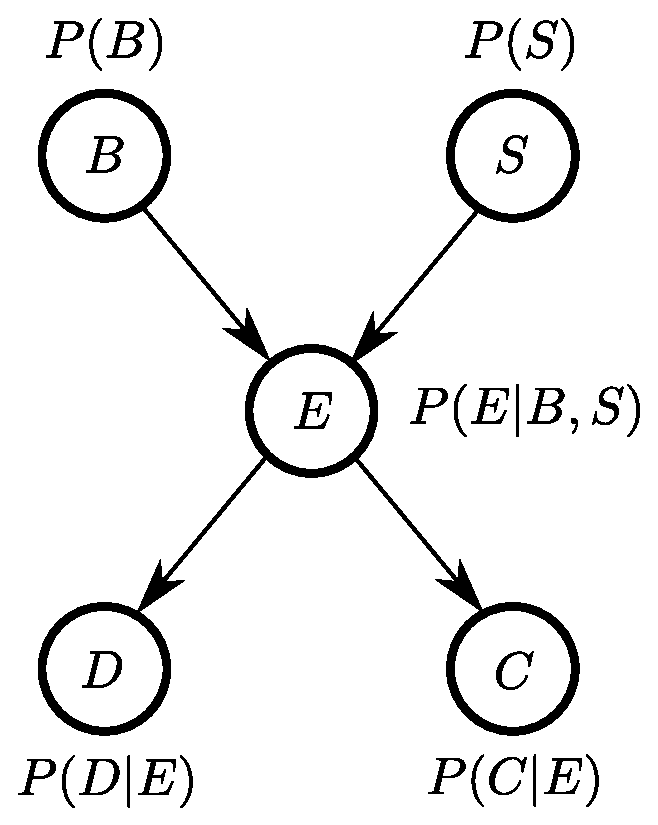
\includegraphics[width=0.8\textwidth]{bn_monitoring.eps}
        \caption{$B$ -- отказ батареи, $S$ -- отказ солнечной панели, $E$ -- отказ системы электропитания, $D$ -- отклонение от траектории, $C$ -- потеря связи.}
    \end{figure}
    \end{minipage}
\end{frame}

\begin{frame}{Цепное правило для байесовской сети}
    \footnotesize

    \begin{itemize}
        \item Цепное правило для байесовской сети определяет построение совместного распределения из локальных распределений условной вероятности.
        \item Пусть в байесовской сети имеются переменные $X_1, \dots, X_n$. Тогда вероятность присвоения им конкретных значений $x_1, \dots, x_n$ имеет вид
        \begin{equation}
            P(x_1, \dots, x_n) = \prod_{i=1}^n P(x_i | pa(x_i)),
        \end{equation}
        где $pa(x_i)$ обозначет присвоение конкретного значения родителю $X_i$.
        \item В нашем примере мы можем захотеть определить вероятность того, что все в порядке, то есть $b = s = e = d = c = 0$:
        \begin{equation}
            \begin{split}
            P(b = 0, s = 0, &e = 0, d = 0, c = 0) = \\
            &P(b = 0) P(s = 0) \times \\
            &P(e = 0 | b = 0, s = 0) \times \\
            &P(d = 0 | e = 0) P(c = 0 | e = 0)
            \end{split}
        \end{equation}
        \item Преимущество байесовской сети состоит в том, что без нее нам бы потребовался $2^5 - 1 = 31$ параметр для задания совместного распределения, а с ней -- только $1 + 1 + 4 + 2 + 2 = 10$
    \end{itemize}
\end{frame}

\begin{frame}{Условная независимость и d-разделение}
    \footnotesize

    \begin{itemize}
        \item Под условной независимостью $X \perp Y | Z$ понимается $P(X, Y | Z) = P(X | Z) P(Y | Z)$, из чего следует $X \perp Y | Z \Longrightarrow P(X | Z, Y) = P(X | Z)$.
        \item В нашем пример $D \perp C | E$: если известно, что произошел сбой питания, информация о потери связи не влияет на вероятность наличия отклонения от траектории.
        \item Байесовская сеть позволяет определить, являются ли две переменные $A, B$ условно независимыми при заданных обусловливающих переменных, используя d-разделение. 
    \end{itemize}
\end{frame}

\begin{frame}{Наивный байесовский классификатор}
    \footnotesize

    \begin{itemize}
        \item \emph{Наивный байесовский классификатор} является простейшим примером байесовской сети.
        \item Он называется ``наивным'', потому что он предполагает условную независимость признаков при данном значении класса.
    \end{itemize}

    Пусть $y$ обозначает класс, а $x_1, \dots, x_n$ признаки. По формуле Байеса:
    \begin{equation}
        P(y | x_1, \dots, x_n) = \frac{P(x_1, \dots, x_n | y) P(y)}{P(x_1, \dots, x_n)}.
    \end{equation}
    Условная независимость признаков подразумевает
    \begin{equation}
        P(x_i | y, x_1, \dots, x_{i-1}, x_{i+1}, \dots, x_n) = P(x_i | y).
    \end{equation}
    Тогда имеем
    \begin{multline}
        P(x_1, \dots, x_n | y) = P(x_2, \dots, x_n | y, x_1) P(x_1 | y) = P(x_2, \dots, x_n | y) P(x_1 | y) = \\
        \dots = \prod_{i = 1}^n P(x_i | y),
    \end{multline}
    что дает
    \begin{equation}
        P(y | x_1, \dots, x_n) = \frac{P(y) \prod_{i = 1}^n P(x_i | y)}{P(x_1, \dots, x_n)}.
    \end{equation}
\end{frame}

\begin{frame}{Наивный байесовский классификатор}
    \footnotesize

    Наивный байесовский классификатор далее рассматривает оценку апостериорного максимума:
    \begin{equation}
        \hat{y} = \text{argmax}_{y} P(y) \prod_{i = 1}^n P(x_i | y).
    \end{equation}
    Для построения классификатора необходимо выбрать априорное распределение $P(y)$ и выбрать параметрическую форму для распределений признаков $P(x_i | y)$.
    
    \begin{itemize}
        \item Пусть $\mathcal{D} = \{(\bm{x}^{(i)}, y_i)\}_{i=1}^n$ 
        \item Априорное распределение: $P(y) = \dfrac{|\{(\bm{x}^{(i)}, y_i) \in \mathcal{D} \ | \ y_i = y\}|}{|\mathcal{D}|}$
        \item Распределение признаков:
        \begin{itemize}
            \footnotesize
            \item Гауссовский наивный Байес: $P(x_i | y) \sim \text{n}(\mu_y, \sigma_y^2)$, где $\mu_y$ и $\sigma_y^2$ оценивается по максимальному правдоподобию.
            \item Мультиномиальный наивный Байес: предлагается, что все признаки являются частотными, то есть $x_i$ обозначает, сколько раз произошло событие $i$ в данном элементе выборки. Тогда $p(x_1, \dots, x_n) = \frac{\sum_{i=1}^n x_i !}{\prod_{i=1}^n x_i !} \prod_{i=1}^n p_{ki}^{x_i}$, где по максимальному правдоподобию можно оценить $p_{ki}$. Используется для классификации документов (метод ``мешка слов'', bag-of-words)
        \end{itemize}
    \end{itemize}
\end{frame}

\end{document}
